\documentclass[runningheads]{llncs}

% ---------------------------------------------------------------
% Include basic ECCV package
 
% TODO REVIEW: Insert your submission number below by replacing '*****'
% TODO FINAL: Comment out the following line for the camera-ready version
% \usepackage[review,year=****,ID=****]{****}
% TODO FINAL: Un-comment the following line for the camera-ready version
\usepackage{eccv}

% OPTIONAL: Un-comment the following line for a version which is easier to read
% on small portrait-orientation screens (e.g., mobile phones, or beside other windows)
%\usepackage[mobile]{****}


% ---------------------------------------------------------------
% Other packages

% Commonly used abbreviations (\eg, \ie, \etc, \cf, \etal, etc.)
\usepackage{eccvabbrv}
% Include other packages here, before hyperref.
\usepackage{graphicx}
\usepackage{booktabs}

% The "axessiblity" package can be found at: https://ctan.org/pkg/axessibility?lang=en
\usepackage[accsupp]{axessibility}  % Improves PDF readability for those with disabilities.


% ---------------------------------------------------------------
% Hyperref package

% It is strongly recommended to use hyperref, especially for the review version.
% Please disable hyperref *only* if you encounter grave issues.
% hyperref with option pagebackref eases the reviewers' job, but should be disabled for the final version.
%
% If you comment hyperref and then uncomment it, you should delete
% main.aux before re-running LaTeX.
% (Or just hit 'q' on the first LaTeX run, let it finish, and you
%  should be clear).

% TODO FINAL: Comment out the following line for the camera-ready version
% \usepackage[pagebackref,breaklinks,colorlinks,citecolor=eccvblue]{hyperref}
% TODO FINAL: Un-comment the following line for the camera-ready version
\usepackage{hyperref}

% Support for ORCID icon
\usepackage{orcidlink}


\begin{document}

% ---------------------------------------------------------------
% TODO REVIEW: Replace with your titlbluee
\title{Champ: Controllable and Consistent Human Image Animation with 3D Parametric Guidance} 

% TODO REVIEW: If the paper title is too long for the running head, you can set
% an abbreviated paper title here. If not, comment out.
\titlerunning{Champ: Controllable Human Image Animation w. 3D Parametric Guidance}

% TODO FINAL: Replace with your author list. 
% Include the authors' OCRID for the camera-ready version, if at all possible.
\author{Shenhao Zhu*\inst{1} \and
Junming Leo Chen*\inst{2} \and
Zuozhuo Dai\inst{3} \and
Qingkun Su\inst{3} \and \\
Yinghui Xu\inst{2} \and
Xun Cao\inst{1} \and 
Yao Yao\inst{1} \and
Hao Zhu$^\dag$\inst{1} \and
Siyu Zhu$^\dag$\inst{2} }

% TODO FINAL: Replace with an abbreviated list of authors.
\authorrunning{S. Zhu et al.}
% First names are abbreviated in the running head.
% If there are more than two authors, 'et al.' is used.

% TODO FINAL: Replace with your institution list.
\institute{Nanjing University, Nanjing, China \and
Fudan University, Shanghai, China \and
Alibaba Group, Hangzhou, China \\
\email{shenhaozhu@smail.nju.edu.cn, leochenjm@gmail.com, \\ \{caoxun, yaoyao, zh\}@nju.edu.cn, zuozhuo.dzz@alibaba-inc.com, \\ suqingkun@gmail.com, \{xuyinghui, siyuzhu\}@fudan.edu.cn}}

\maketitle

\begin{abstract}
In this study, we introduce a methodology for human image animation by leveraging a 3D human parametric model within a latent diffusion framework to enhance shape alignment and motion guidance in curernt human generative techniques.
The methodology utilizes the SMPL(Skinned Multi-Person Linear) model as the 3D human parametric model to establish a unified representation of body shape and pose. 
This facilitates the accurate capture of intricate human geometry and motion characteristics from source videos.
Specifically, we incorporate rendered depth images, normal maps, and semantic maps obtained from SMPL sequences, alongside skeleton-based motion guidance, to enrich the conditions to the latent diffusion model with comprehensive 3D shape and detailed pose attributes.
A multi-layer motion fusion module, integrating self-attention mechanisms, is employed to fuse the shape and motion latent representations in the spatial domain.
By representing the 3D human parametric model as the motion guidance, we can perform parametric shape alignment of the human body between the reference image and the source video motion. 
Experimental evaluations conducted on benchmark datasets demonstrate the methodology's superior ability to generate high-quality human animations that accurately capture both pose and shape variations. 
Furthermore, our approach also exhibits superior generalization capabilities on the proposed in-the-wild dataset. Project page: \url{https://fudan-generative-vision.github.io/champ}.

\keywords{Latent Diffusion Model \and Human Image Animation \and 3D human parametric model \and Motion Guidance}
\end{abstract}
\let\thefootnote\relax\footnotetext{$^*$ These authors contributed equally to this work.}
\let\thefootnote\relax\footnotetext{ $^\dag$ Corresponding Author}
\section{Introduction}
\label{sec:intro}

\begin{figure*}[t]
\centering
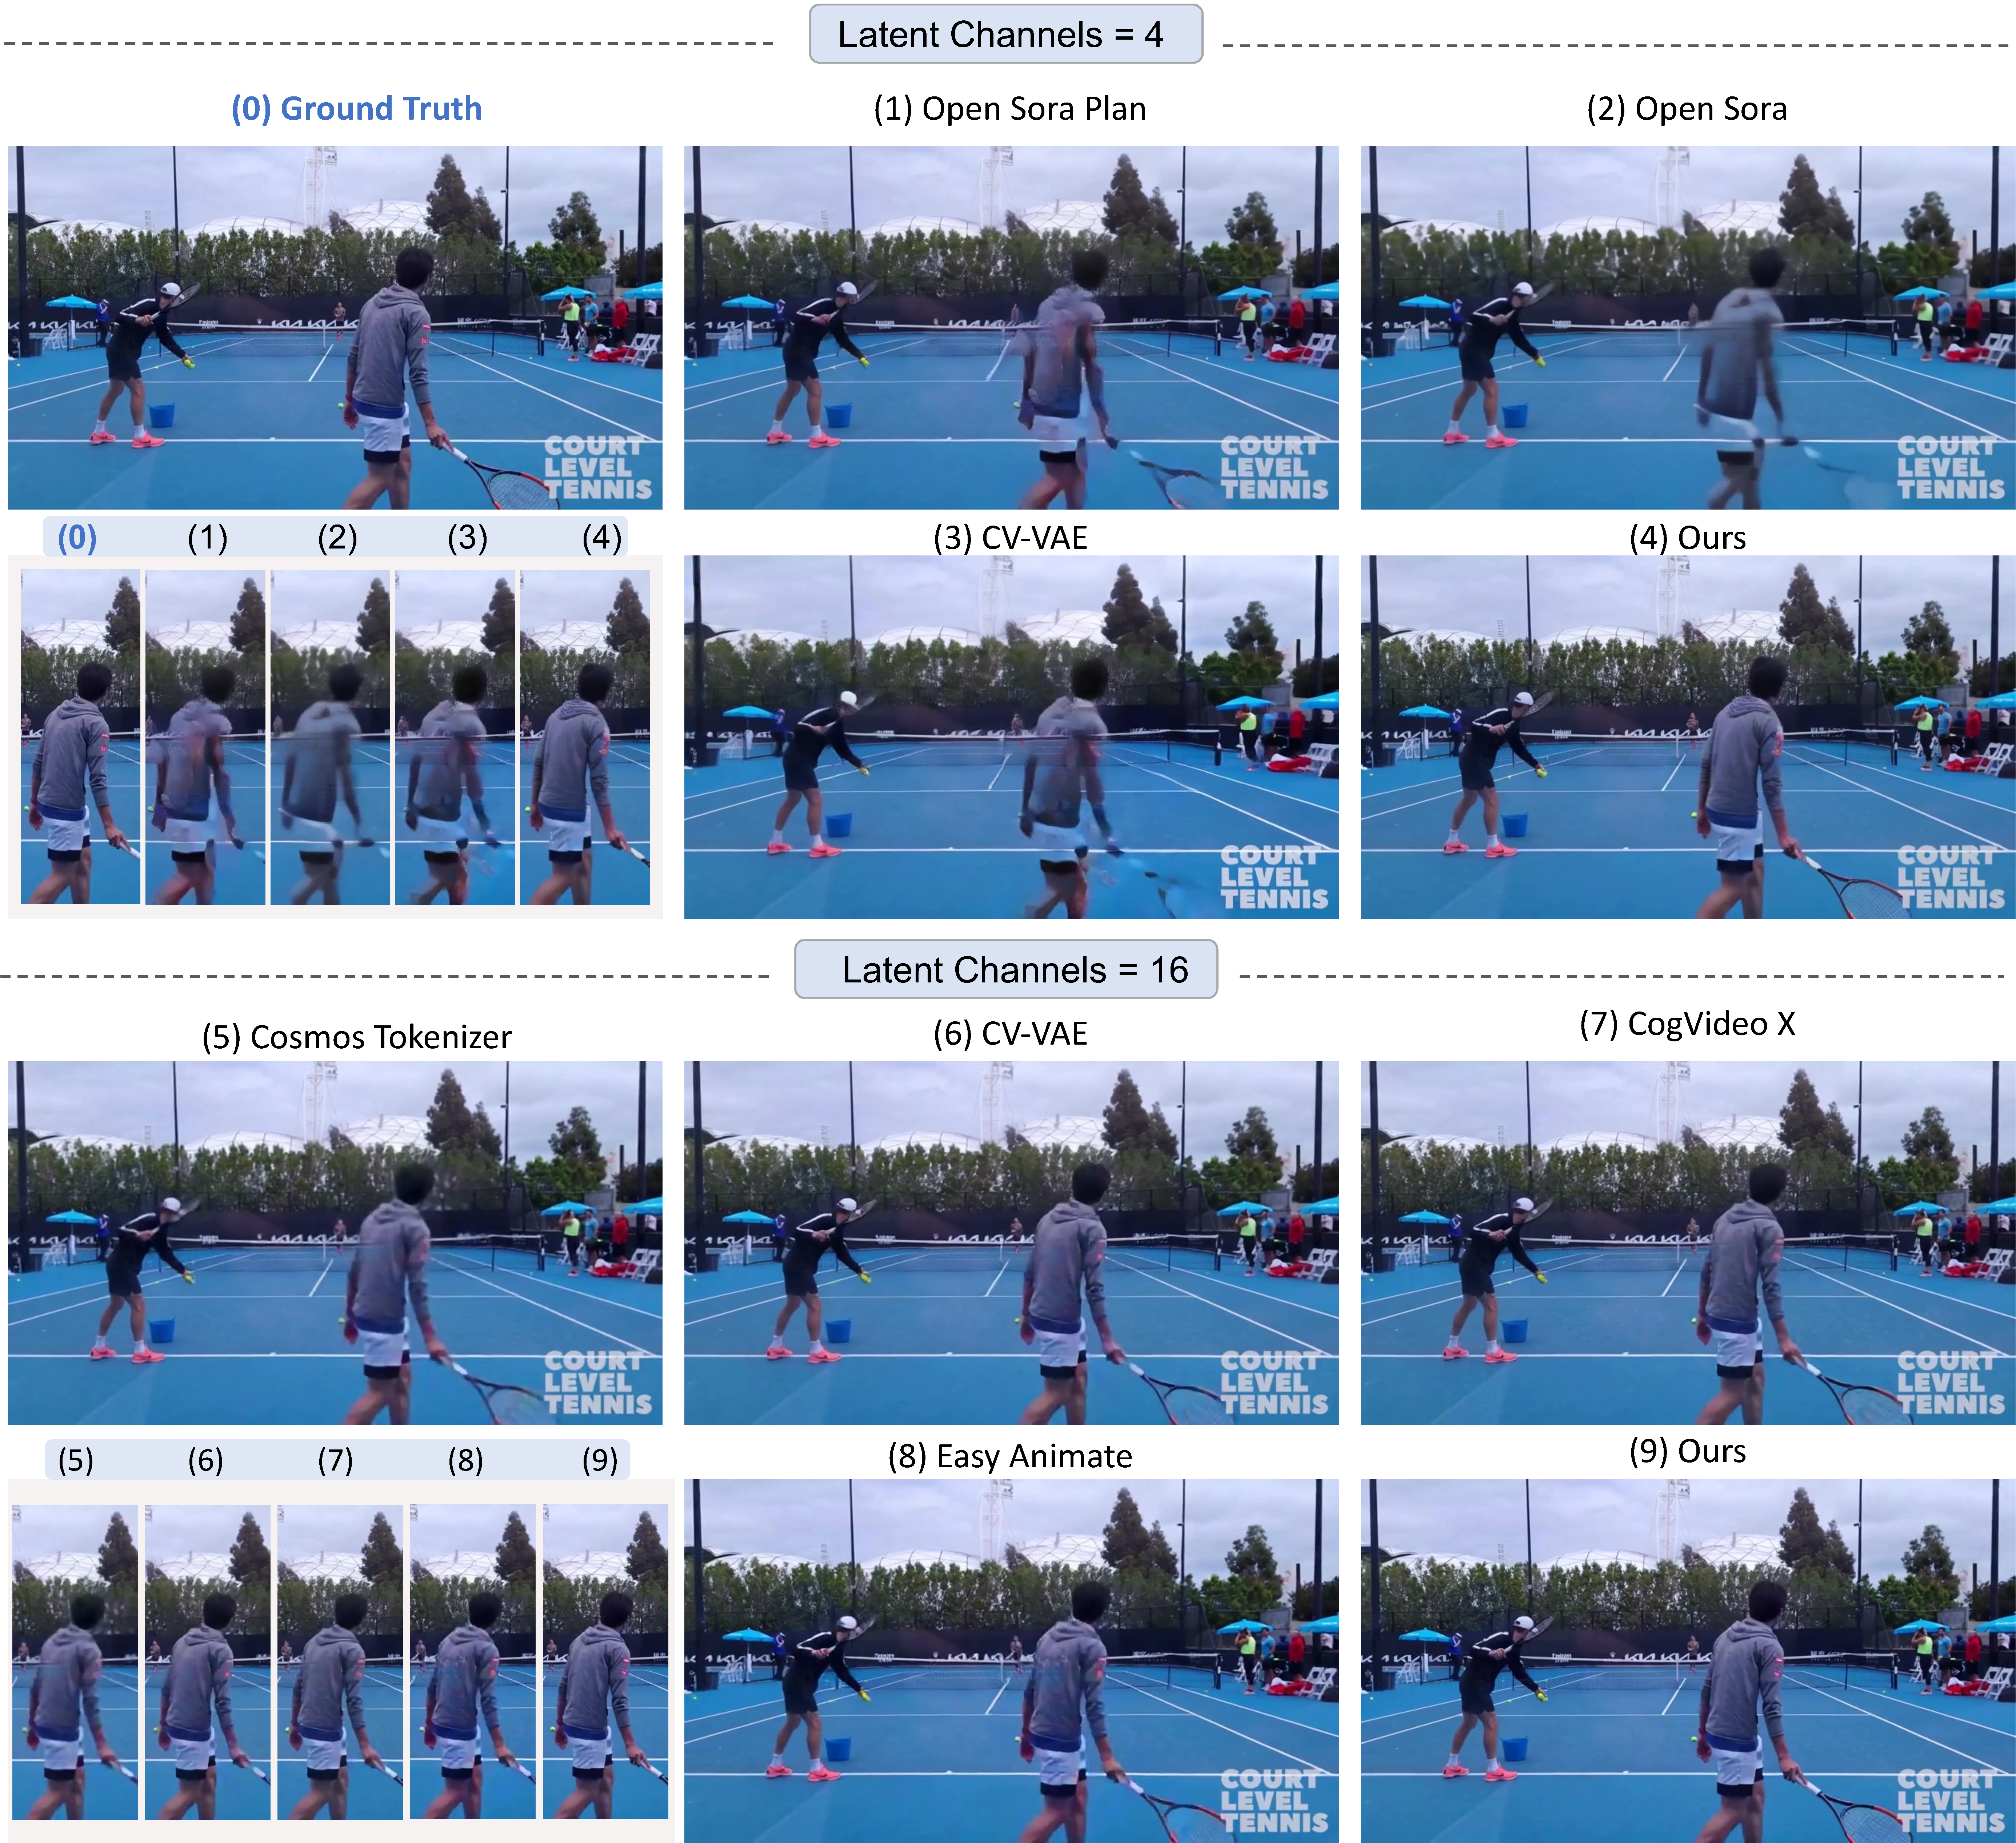
\includegraphics[width=1.0\textwidth]{images/fig1-4and16.pdf}
\caption{
Our reconstruction results compared with a line of three recent strong baseline approaches. 
The ground truth frame is (0). Our model significantly outperforms previous methods, especially under large motion scenarios such as people doing sports.
}
\label{fig:teaser}
\vspace{-3mm}
\end{figure*}



Given the significant attention in the field of video generation, Latent Video Diffusion Models (LVDMs)~\cite{blattmann2023stable, blattmann2023align, he-lvdm, zhou2022magicvideo, he-videocrafter1} have emerged as a popular framework. They have been successfully applied to powerful text-to-video models such as Sora~\cite{videoworldsimulators2024}, VideoCrafter~\cite{he-videocrafter1, chen2024videocrafter2overcomingdatalimitations}, and CogVideoX~\cite{yang2024cogvideox}.
Different from directly generating video pixels, LVDMs generate latent video representations in a compact latent space. This is achieved by first training a Video VAE to encode videos into this latent space.
%
Thus, Video VAE, as a key and fundamental component of LVDMs, has attracted great attention recently.
%
An effective Video VAE can help to reduce the training costs of video diffusion models while improving the final quality of the generated videos.
%
Initially, a series of studies adopt the image VAE from Stable Diffusion~\cite{rombach2022high} for video generation tasks, including AnimateDiff~\cite{guoanimatediff}, MagicVideo~\cite{zhou2022magicvideo}, VideoCrafter1~\cite{he-videocrafter1}, and VideoCrafter2~\cite{chen2024videocrafter2overcomingdatalimitations}. 
%
However, directly adopting an image VAE and compressing video on a frame-by-frame basis leads to temporal flickering due to the lack of temporal correlation. Additionally, the information redundancy along the temporal dimension is not reduced, leading to low training efficiency for subsequent latent video diffusion models.
%
From the introduction of Sora, which compresses videos both temporally and spatially through a Video VAE, a series of studies have emerged that aim to replicate Sora and train their own Video VAEs, including Open Sora~\cite{opensora}, Open Sora Plan~\cite{pku_yuan_lab_and_tuzhan_ai_etc_2024_10948109}, CV-VAE~\cite{zhao2024cv}, CogVideoX~\cite{yang2024cogvideox}, EasyAnimate~\cite{xu2024easyanimatehighperformancelongvideo}, and Cosmos Tokenizer~\cite{cosmos_token}.
%
However, the performance of the current video VAE suffers from many problems, including motion ghost, low-level temporal flickering, blurring (faces, hands, edges, texts), and motion stuttering (lack of correct temporal transition).
% as shown in Fig.~\ref{fig:teaser}.


In this work, we propose a novel cross-modal Video VAE with better spatial and temporal modeling ability in order to solve the aforementioned challenge problems and obtain a robust and high-quality Video VAE.
%
First, we examine different designs for spatial and temporal compression, including simultaneous spatial-temporal (ST) compression and sequential ST compression. 
%
We observed that simultaneous ST compression achieves better low-level temporal smoothness and texture stability, while sequential ST compression achieves better motion recovery, particularly in scenarios of large motion.
%
Thus, we propose a novel architecture that integrates the advantages of both methods and enables effective video detail and motion reconstruction.

Second, we observed that the normally used datasets for text-to-video generation contain text-video pairs. 
Also, during decoding, a text description exists as it serves as the input in the first stage, \textit{i.e.}, the video latent generation stage.
%
To this end, we integrate the text information into the encoding and decoding procedure and propose the first Cross-modal Video VAE.
%
We carefully study how text guidance can be integrated into the spatiotemporal backbone and the mechanism of spatial and temporal semantic guidance. 

In addition, our cross-modal video VAE supports image-video joint training.
To achieve this, we design our network with a fully spatiotemporal factorized architecture, and we feed image and video batches alternately to the network. 
%
During image batches, the data only forwards the spatial part of the network, with the temporal modules being skipped. During video batches, the video forwards both spatial and temporal modules. We also demonstrate that image joint training is crucial for training a video VAE.
%
In summary, our contributions are as follows:
\begin{itemize}
    \item We propose an effective and robust Video VAE, conduct extensive experiments, and achieve the state-of-the-art.
    \item We propose an optimal spatiotemporal modeling approach for Video VAE.
    \item We propose the first cross-modal video VAE that leverages the information from other modalities, i.e., text descriptions, to the best of our knowledge.
    \item Our video VAE is designed and trained to be versatile to conduct both image and video compression. 
\end{itemize}


% \vspace{-2mm}
\section{Related Work}
% \vspace{-2mm}
\label{sec:formatting}
%We now review relevant works on segmentation, vision transformers, and efficient attention.

%-------------------------------------------------------------------------
% \subsection{Video Object Segmentation}
{\bf Video Object Segmentation (VOS)} is a fundamental task in computer vision, segments objects of interest from the background and tracks target objects in a video. 
%Many research works have been proposed in this community on video object segmentation. 
In the unsupervised setting~\citep{grundmann2010efficient,brox2010object,lee2011key,xu2012evaluation,fragkiadaki2012video,perazzi2012saliency,zhang2013video,li2013video,papazoglou2013fast,faktor2014video,wang2015saliency,taylor2015causal,perazzi2016benchmark}, VOS models segment salient objects without a reference mask. In the semi-supervised setting~\citep{pont20172017,xu2018youtube,oh2019video,bhat2020learning,robinson2020learning,li2022recurrent,yang2022decoupling,cheng2022xmem,zhang2023joint,wang2023look,wu2023scalable,cheng2024putting,yang2024scalable}, VOS requires tracking and segmenting objects based on a first-frame mask of target objects. For interactive video object segmentation (iVOS)~\citep{caelles20182018,heo2020interactive,cheng2021modular,homayounfar2021videoclick,yang2023track,cheng2023segment,rajivc2023segment,cheng2024putting,delatolas2024learning}, iVOS models perform object segmentation in videos (masklets) with user guidance, e.g., clicks, bounding boxes, scribbles. In SAM 2~\citep{ravi2024sam}. Semi-supervised VOS and iVOS have been extended to promptable visual segmentation (PVS), where the model can be interactively prompted with different types of inputs such as clicks, boxes, and masks on any frame in a video for segmenting and tracking a valid object.
%-------------------------------------------------------------------------

% \subsection{Vision Transformers}
\noindent {\bf Vision Transformers (ViTs)} have achieved huge success on various vision tasks including image classification~\citep{dosovitskiy2020image}, object detection~\citep{li2022exploring}, image segmentation~\cite{cheng2022masked,kirillov2023segment}, video classification~\citep{fan2021multiscale}, and video object segmentation~\citep{duke2021sstvos,yang2023track}. The original ViT family scales from the efficient ViT-Tiny up to ViT-Huge, with a plain, non-hierarchical architecture. There are also hierarchical vision transformers that combine transformers with hierarchical stage structure, such as Swin~\citep{liu2021swin}, MViT~\citep{fan2021multiscale,li2022mvitv2}, PViT~\citep{wang2021pyramid}, and Hiera~\citep{ryali2023hiera}. While being successful, hierarchical models are usually slower than their plain ViT counterparts for practical deployment~\citep{ryali2023hiera}. 
Combining ViT with convolutions~\citep{lecun1989backpropagation} has been explored for fast hybrid models such as MobileViT~\citep{mehta2021mobilevit}, LeViT~\citep{graham2021levit},  EfficientFormer\citep{li2022efficientformer}, Next-ViT\citep{li2022next}, Tiny-ViT\citep{wu2022tinyvit}, Castling-ViT\citep{you2023castling}, EfficientViT~\citep{liu2023efficientvit}, and MobileNetv4~\citep{qin2024mobilenetv4}. This line of progression towards building efficient ViTs is orthogonal to our
EfficientTAM work towards building efficient video object segmentation. Following SAM~\citep{kirillov2023segment} and EfficientSAMs~\citep{xiong2024efficientsam}, we are pursuing plain ViT backbones for efficient video object segmentation and track anything tasks.  
%The community has also shown increasing interest in efficient vision transformers; \citep{touvron2021training} presented smaller ViTs such as ViT-Small and ViT-Tiny for complementing ViT-Huge, ViT-Large, and ViT-Base in \citep{dosovitskiy2020image}. 


%-------------------------------------------------------------------------
% \subsection{Efficient Attention}
\noindent {\bf Efficient Attention.} The field has developed methods to reduce the quadratic cost of standard self-attention with respect to input sequence length~\cite{attention_is_all_you_need}. 
Local windowed attention has been applied in \cite{beltagy2020longformer,zaheer2020bigbird} for reducing the complexity of self-attention. In \cite{shen2018efficient,katharopoulos-et-al-2020}, a linear dot product approximation is proposed to linearize the softmax matrix in self-attention by heuristically separating keys and queries. In \cite{choromanski2020rethinking}, the Performer model uses random features to approximate self-attention, achieving linear time and memory cost. Nystr\"{o}mformer in \cite{xiong2021nystromformer} makes use of the Nystr\"{o}m method to approximate self-attention with a linear cost. Linformer \cite{wang2020linformer} shows that self-attention is low-rank, which can be approximated by learning linear projection matrices for the keys and values. The approach of~\citep{liu2023efficientvit,you2023castling} leverages the associative property of matrix multiplication for efficient attentions in vision transformers. This direction has shown success and has achieved decent performance on vision tasks. However, in preliminary experiments we found that these methods underperformed in a memory cross-attention module when adapted for efficiency improvement.


%-------------------------------------------------------------------------
% \subsection{Segment Anything Model}
\noindent {\bf Segment Anything Model.} SAM~\citep{kirillov2023segment} is a vision foundation model that can segment any object in an image using interactive prompts such as points and bounding boxes. SAM has demonstrated remarkable zero-shot transfer performance and high versatility for many vision tasks including a broad range of segmentation applications~\citep{chen2023semantic,cen2023sad,deng2023segment,chen2023sam}, in-painting~\citep{yu2023inpaint}, image restoration~\citep{jiang2023restore}, image editing~\citep{gao2023editanything}, image shadow removal~\citep{zhang2023deshadow}, medical image segmentation~\citep{ma2023segment}, camouflaged object detection~\citep{tang2023can}, transparent object detection~\citep{han2023segment}, concept-based explanation~\citep{sun2023explain}, semantic communication~\citep{tariq2023segment}, and object tracking~\citep{cheng2023segment,yang2023track}. The strong ability on image segmentation with flexible prompts motivates the extension of SAM for video object segmentation and track anything. Track Anything Model (TAM)~\citep{yang2023track} combines SAM and XMem~\cite{cheng2022xmem} for interactive video object tracking and segmentation with SAM for frame segmentation and XMem for tracking. SAM-Track~\citep{cheng2023segment} perform object tracking and segmentation in videos by combining SAM~\citep{kirillov2023segment}, DeAOT~\citep{yang2022decoupling}, and Grounding-Dino~\citep{liu2023grounding}. The latest SAM 2~\citep{ravi2024sam} extended SAM for video segmentation through a hierarchical image encoder for frame embeddings and a memory module that conditions current frame embeddings on past frames. Motivated by mobile app use-cases and computationally-constrained applications, recent works have reduced the computational cost of SAM, such as MobileSAM~\citep{zhang2023faster}, FastSAM~\citep{zhao2023fast}, and EfficientSAM~\citep{xiong2024efficientsam}.
The present paper focuses on improving the efficiency challenges of SAM 2 for practical deployment of video object segmentation and track anything.  
\section{Method}
\label{sec:method}

\subsection{Practical choice of diffusion paradigm}
\label{subsec:practical_dwm}

Building on the background provided in Section \ref{sec:framework}, we now introduce \textsc{diamond} as a practical realization of a diffusion-based world model. In particular, we now define the drift and diffusion coefficients $\mathbf{f}$ and $g$ introduced in Section \ref{subsec:diffusion}, corresponding to a particular choice of diffusion paradigm. While \textsc{ddpm} \citep{ho2020DDPM} is an example of one such choice (as described in Appendix \ref{app:ddpm}) and would historically be the natural candidate, we instead build upon the \textsc{edm} formulation proposed in \citet{karras2022elucidating}. The practical implications of this choice are discussed in Section \ref{subsec:diffusion_choice}. In what follows, we describe how we adapt \textsc{edm} to build our diffusion-based world model.

We consider the perturbation kernel $p^{0\tau}(\x_{t+1}^\tau \mid \x_{t+1}^0) = \mathcal{N}(\x_{t+1}^\tau; \x_{t+1}^0, \sigma^2(\tau) \mathbf{I})$, where $\sigma(\tau)$ is a real-valued function of diffusion time called the noise schedule. This corresponds to setting the drift and diffusion coefficients to $\mathbf{f}(\x, \tau) = \mathbf{0}$ (affine) and $g(\tau) = \sqrt{2 \dot \sigma(\tau) \sigma(\tau)}$.

We use the network preconditioning introduced by \citet{karras2022elucidating} and so parameterize $\mathbf{D}_\theta$ in Equation \ref{eq:denoising_sm_conditional} as the weighted sum of the noised observation and the prediction of a neural network $\mathbf{F}_\theta$,
\begin{equation}
\label{eq:karras_wrappers} 
    \mathbf{D}_\theta(\x_{t+1}^\tau, y_t^\tau) = c_\text{skip}^\tau \; \x_{t+1}^\tau + c_\text{out}^\tau \; \mathbf{F}_\theta \big( c_\text{in}^\tau \; \x_{t+1}^\tau, y_t^\tau \big),
\end{equation}
where for brevity we define $y_t^\tau \coloneqq (c_\text{noise}^\tau, \x^0_{\le t}, a_{\le t})$ to include all conditioning variables.

The preconditioners $c_\text{in}^\tau$ and $c_\text{out}^\tau$ are selected to keep the network's input and output at unit variance for any noise level $\sigma(\tau)$, $c_\text{noise}^\tau$ is an empirical transformation of the noise level, and $c_\text{skip}^\tau$ is given in terms of $\sigma(\tau)$ and the standard deviation of the data distribution $\sigma_\text{data}$, as $c_{skip}^\tau = \sigma_{data}^2/(\sigma_{data}^2 + \sigma^2(\tau))$. These preconditioners are fully described in Appendix \ref{appendix:karras_conditioners}.

Combining Equations \ref{eq:denoising_sm_conditional} and \ref{eq:karras_wrappers} provides insight into the training objective of $\mathbf{F}_\theta$,
\begin{align}
\label{eq:effective_obj}
\mathcal{L}(\theta)  = \bbe \Big[ \Vert 
\underbrace{\mathbf{F}_\theta \big( c_\text{in}^\tau \x_{t+1}^\tau, y_t^\tau \big)}_\text{Network prediction} - 
\underbrace{\frac{1}{c_\text{out}^\tau} \big( \x_{t+1}^0 - c_\text{skip}^\tau \x_{t+1}^\tau\big)}_\text{Network training target}
\Vert^2 \Big].
\end{align}
The network training target adaptively mixes signal and noise depending on the degradation level $\sigma(\tau)$.
When $\sigma(\tau) \gg \sigma_\text{data}$, we have $c_\text{skip}^\tau \to 0$, and the training target for $\mathbf{F}_\theta$ is dominated by the clean signal $\x_{t+1}^0$. Conversely, when the noise level is low, $\sigma(\tau) \to 0$, we have $c_\text{skip}^\tau \to 1$, and the target becomes the difference between the clean and the perturbed signal, i.e. the added Gaussian noise. Intuitively, this prevents the training objective to become trivial in the low-noise regime. In practice, this objective is high variance at the extremes of the noise schedule, so \citet{karras2022elucidating} sample the noise level $\sigma(\tau)$ from an empirically chosen log-normal distribution in order to concentrate the training around medium-noise regions, as described in Appendix \ref{appendix:karras_conditioners}.

We use a standard U-Net 2D for the vector field $\mathbf{F}_\theta$ \citep{ronneberger2015unet}, and we keep a buffer of $L$ past observations and actions that we use to condition the model. We concatenate these past observations to the next noisy observation channel-wise, and we input actions through adaptive group normalization layers \citep{adagn} in the residual blocks \citep{He2015} of the U-Net.

As discussed in Section \ref{subsec:dwm_training} and Appendix \ref{appendix:sampling}, there are many possible sampling methods to generate the next observation from the trained diffusion model. While our codebase supports a variety of sampling schemes, we found Euler's method to be effective without incurring the cost of additional NFE required by higher order samplers, or the unnecessary complexity of stochastic sampling.

\subsection{Reinforcement learning in imagination}
\label{subsec:rl}

Given the diffusion model from Section \ref{subsec:practical_dwm}, we now complete our world model with a reward and termination model, required for training an RL agent in imagination. Since estimating the reward and termination are scalar prediction problems, we use a separate model $R_\psi$ consisting of standard \textsc{cnn} \citep{cnn_lecun,He2015} and \textsc{lstm} \citep{lstm,Gers2000} layers to handle partial observability. The RL agent involves an actor-critic network parameterized by a shared \textsc{cnn-lstm} with policy and value heads. The policy $\pi_\phi$ is trained with \textsc{reinforce} with a value baseline, and we use a Bellman error with $\lambda$-returns to train the value network $V_\phi$, similar to \citet{iris2023}. We train the agent entirely in imagination as described in Section \ref{subsec:pomdp_and_wm}. The agent only interacts with the real environment for data collection. After each collection stage, the current world model is updated by training on all data collected so far. Then, the agent is trained with RL in the updated world model environment, and these steps are repeated. This procedure is detailed in Algorithm \ref{alg:diamond}, and is similar to \citet{kaiser2019atari100k,hafner2020dream,iris2023}. We provide architecture details, hyperparameters, and RL objectives in Appendices \ref{app:architectures}, \ref{app:hyperparams}, \ref{appendix:rl_actor_critic}, respectively.

\section{Experiments}
\label{sec:exp}

\begin{table}[t]
\small\centering\setlength{\tabcolsep}{3pt}
\begin{tabular}{l | c | g | g g g g }
\toprule
\rowcolor{white} \textbf{ImageNet 256$\times$256} & Latent Shape & Autoencoder & rFID $\downarrow$ & PSNR $\uparrow$ & SSIM $\uparrow$ & LPIPS $\downarrow$ \\
\midrule
\rowcolor{white} \multirow{2}{*}{f32c32} & \multirow{2}{*}{8$\times$8$\times$32} 
 & SD-VAE \tablecite{rombach2022high} & 2.64 & 22.13 & 0.59 & 0.117 \\
 & & \modelshort                      & \textbf{0.69} & \textbf{23.85} & \textbf{0.66} & \textbf{0.082} \\
\midrule
\rowcolor{white} \multirow{2}{*}{f64c128} & \multirow{2}{*}{4$\times$4$\times$128}
 & SD-VAE \tablecite{rombach2022high} & 26.65 & 18.07 & 0.41 & 0.283 \\
 & & \modelshort                      & \textbf{0.81} & \textbf{23.60} & \textbf{0.65} & \textbf{0.087} \\
\bottomrule
\toprule
\rowcolor{white} \textbf{ImageNet 512$\times$512} & Latent Shape & Autoencoder & rFID $\downarrow$ & PSNR $\uparrow$ & SSIM $\uparrow$ & LPIPS $\downarrow$ \\
 \midrule
\rowcolor{white} \multirow{2}{*}{f64c128} & \multirow{2}{*}{8$\times$8$\times$128}
 & SD-VAE \tablecite{rombach2022high} & 16.84 & 19.49 & 0.48 & 0.282 \\
 & & \modelshort                      & \textbf{0.22} & \textbf{26.15} & \textbf{0.71} & \textbf{0.080} \\
\midrule
\rowcolor{white} \multirow{2}{*}{f128c512} & \multirow{2}{*}{4$\times$4$\times$512}
 & SD-VAE \tablecite{rombach2022high} & 100.74 & 15.90 & 0.40 & 0.531 \\
 & & \modelshort                      & \textbf{0.23} & \textbf{25.73} & \textbf{0.70} & \textbf{0.084} \\
\bottomrule
\toprule
\rowcolor{white} \textbf{FFHQ 1024$\times$1024} & Latent Shape & Autoencoder & rFID $\downarrow$ & PSNR $\uparrow$ & SSIM $\uparrow$ & LPIPS $\downarrow$ \\
\midrule
\rowcolor{white} \multirow{2}{*}{f64c128} & \multirow{2}{*}{16$\times$16$\times$128}
 & SD-VAE \tablecite{rombach2022high} & 6.62 & 24.55 & 0.68 & 0.237 \\
 & & \modelshort                      & \textbf{0.23} & \textbf{31.04} & \textbf{0.83} & \textbf{0.061} \\
 \midrule
\rowcolor{white} \multirow{2}{*}{f128c512} & \multirow{2}{*}{8$\times$8$\times$512}
 & SD-VAE \tablecite{rombach2022high} & 179.71 & 18.11 & 0.63 & 0.585 \\
 & & \modelshort                      &  \textbf{0.41} & \textbf{31.18} & \textbf{0.83} & \textbf{0.062} \\
\bottomrule
\toprule
\rowcolor{white} \textbf{MapillaryVistas 2048$\times$2048} & Latent Shape & Autoencoder & rFID $\downarrow$ & PSNR $\uparrow$ & SSIM $\uparrow$ & LPIPS $\downarrow$ \\ 
 \midrule
\rowcolor{white} \multirow{2}{*}{f64c128} & \multirow{2}{*}{32$\times$32$\times$128}
 & SD-VAE \tablecite{rombach2022high} & 7.55 & 22.37 & 0.68 & 0.262 \\
 & & \modelshort                      & \textbf{0.36} & \textbf{29.57} & \textbf{0.84} & \textbf{0.075} \\
 \midrule
\rowcolor{white} \multirow{2}{*}{f128c512} & \multirow{2}{*}{16$\times$16$\times$512} 
 & SD-VAE \tablecite{rombach2022high} & 152.09 & 17.82 & 0.67 & 0.594 \\
 & & \modelshort                      &  \textbf{0.38} & \textbf{29.70} & \textbf{0.84} & \textbf{0.074} \\
\bottomrule
\end{tabular}
\vspace{-5pt}
\caption{\textbf{Image Reconstruction Results.}}
\vspace{-10pt}
\label{tab:ae_main}
\end{table}

\subsection{Setups}

\paragraph{Implementation Details.} We use a mixture of datasets to train autoencoders (baselines and \modelshort), containing ImageNet \citep{deng2009imagenet}, SAM \citep{kirillov2023segment}, MapillaryVistas \citep{neuhold2017mapillary}, and FFHQ \citep{karras2019style}. For ImageNet experiments, we exclusively use the ImageNet training split to train autoencoders and diffusion models. The model architecture is similar to SD-VAE \citep{rombach2022high} except for our new designs discussed in Section~\ref{sec:main_model}. In addition, we use the original autoencoders instead of the variational autoencoders for our models, as they perform the same in our experiments and the original autoencoders are simpler. We also replace transformer blocks with EfficientViT blocks \citep{cai2023efficientvit} to make autoencoders more friendly for handling high-resolution images while maintaining similar accuracy. 

For image generation experiments, we apply autoencoders to diffusion transformer models including DiT \citep{peebles2023scalable} and UViT \citep{bao2023all}. We follow the same training settings as the original papers. 
We consider three settings with different resolutions, including ImageNet \citep{deng2009imagenet} for $512 \times 512$ generation, FFHQ \citep{karras2019style} and MJHQ \citep{li2024playground} for $1024 \times 1024$ generation, and MapillaryVistas \citep{neuhold2017mapillary} for $2048 \times 2048$ generation. 

\begin{table}[t]
\small\centering\setlength{\tabcolsep}{2pt}
\begin{tabular}{l | g | g | g g | g | g | g g }
\toprule
\rowcolor{white} Diffusion & & Patch & \multicolumn{2}{c|}{Throughput (image/s) $\uparrow$} & Latency & Memory & \multicolumn{2}{c}{FID $\downarrow$} \\
\rowcolor{white} Model & \multirow{-2}{*}{Autoencoder} & Size & Training & Inference & (ms) $\downarrow$ & (GB) $\downarrow$ & w/o CFG & w/ CFG \\
\midrule
\rowcolor{white} & SD3-VAE-f8 \tablecite{esser2024scaling}                   & 2 &  352 &  2984 & 3.8 & 13.8 & 164.34 & 143.82 \\
\rowcolor{white} & Flux-VAE-f8 \tablecite{flux2024}                          & 2 &  352 &  2984 & 3.8 & 13.8 & 106.07 & 84.73 \\
\cmidrule{2-9}
\rowcolor{white} & SDXL-VAE-f8 \tablecite{podell2023sdxl}                    & 2 &  352 &  2991 & 3.8 & 13.8 & 51.03 & 26.38 \\
\rowcolor{white} & Asym-VAE-f8 \tablecite{zhu2023designing}                  & 2 &  352 &  2991 & 3.8 & 13.8 & 51.96 & 24.57 \\
\rowcolor{white} & SD-VAE-f8 \tablecite{rombach2022high}                     & 2 &  352 &  2991 & 3.8 & 13.8 & 51.96 & 24.57 \\
\rowcolor{white} & SD-VAE-f16 \tablecite{rombach2022high}                    & 2 & 1550 & 12881 & 1.3 &  4.0 & 76.86 & 44.22 \\
\rowcolor{white} & SD-VAE-f32 \tablecite{rombach2022high}                    & 1 & 1551 & 12883 & 1.3 &  4.0 & 70.23 & 38.63 \\
\cmidrule{2-9}
& \modelshort-f32                                                            & 1 & 1553 & 12850 & 1.3 &  4.0 & \textbf{46.12} & \textbf{18.08} \\ 
& \modelshort-f64                                                            & 1 & \textbf{6295} & \textbf{53774} & \textbf{0.7} & \textbf{1.5} & 67.30 & 35.96 \\
\multirow{-11}{*}{UViT-S \tablecite{bao2023all}} & \:\:\modelshort-f64$^\dag$ & 1 & \textbf{6295} & \textbf{53774} & \textbf{0.7} & \textbf{1.5} & 61.84 & 30.63 \\
\midrule
\midrule
\rowcolor{white} & Flux-VAE-f8 \tablecite{flux2024}                          & 2 &   54 &  416 & 31.7 & 56.3 & 27.35 & 8.72 \\
\cmidrule{2-9}
\rowcolor{white} & Asym-VAE-f8 \tablecite{zhu2023designing}                  & 2 &   54 &  424 & 31.7 & 56.2 & 11.55 & 2.95 \\
\rowcolor{white} &  SD-VAE-f8 \tablecite{rombach2022high}                    & 2 &   54 &  424 & 31.7 & 56.2 & 12.03 & 3.04 \\
\cmidrule{2-9}
& \modelshort-f32                                                            & 1 &  \textbf{241} &  \textbf{2016} & \textbf{7.8} & \textbf{20.9} &  9.56 & 2.84 \\
\multirow{-5}{*}{DiT-XL \tablecite{peebles2023scalable}} 
& \:\:\modelshort-f32$^\ddag$                                                    & 1 &  \textbf{241} &  \textbf{2016} & \textbf{7.8} & \textbf{20.9} &  \textbf{6.88} & \textbf{2.41} \\


\midrule
\midrule
\rowcolor{white} & Flux-VAE-f8 \tablecite{flux2024}                          & 2 &  55 &  349 & 30.4 & 54.2 & 30.91 & 12.63 \\
\cmidrule{2-9}
\rowcolor{white} & Asym-VAE-f8 \tablecite{zhu2023designing}                  & 2 &  55 &  351 & 30.3 & 54.1 & 11.36 &  3.51 \\
\rowcolor{white}  & SD-VAE-f8 \tablecite{rombach2022high}                    & 2 &   \,\,55\,\,\tikzmark{uvit_h_f8p2:a1} &   \,\,351\,\,\tikzmark{uvit_h_f8p2:a2} & 30.3 & 54.1 & 11.04 & \,\,3.55\,\,\tikzmark{uvit_h_f8p2:a3} \\
\cmidrule{2-9}
& \modelshort-f32                                                            & 1 &  247 &  1622 &  8.2 & 18.6 &  \textbf{9.83} & \textbf{2.53} \\
& \modelshort-f64                                                            & 1 & \,\,\textbf{984}\,\,\tikzmark{uvit_h_f64p1:a1} &  \,\,\textbf{6706}\,\,\tikzmark{uvit_h_f64p1:a2} & \textbf{3.5} & \textbf{10.6} & 13.96 & \,\,3.01\,\,\tikzmark{uvit_h_f64p1:a3} \\
\multirow{-6}{*}{UViT-H \tablecite{bao2023all}} & \:\:\modelshort-f64$^\dag$ & 1 & \textbf{984} &  \textbf{6706} & \textbf{3.5} & \textbf{10.6} & 12.26 & 2.66 \\

\midrule
\midrule
\rowcolor{white} & Asym-VAE-f8 \tablecite{zhu2023designing}                   & 2 &  27 & 157 & 74.8 & OOM & 9.87 & 3.62 \\
\rowcolor{white}  & SD-VAE-f8 \tablecite{rombach2022high}                     & 2 &  27 & 157 & 74.8 & OOM & 9.73 & 3.57 \\
\cmidrule{2-9}
& \modelshort-f32                                                             & 1 & 112 & 665 & 19.7 & 42.0 & 8.13 & 2.30 \\
& \modelshort-f64                                                             & 1 & \textbf{450} & \textbf{2733} & \textbf{8.6} & \textbf{30.2} & 7.78 & 2.47 \\
\multirow{-5}{*}{UViT-2B \tablecite{bao2023all}} & \:\:\modelshort-f64$^\dag$ & 1 & \textbf{450} & \textbf{2733} & \textbf{8.6} & \textbf{30.2} & \textbf{6.50} & \textbf{2.25} \\

\bottomrule
\end{tabular}

\begin{tikzpicture}[overlay, remember picture, shorten >=.5pt, shorten <=.5pt, transform canvas={yshift=.25\baselineskip}]

\draw [->, red] ({pic cs:uvit_h_f8p2:a1}) [bend left] to node [below right] (uvit_h_f8p2:t1) {\hspace{-2pt}\scriptsize \textbf{17.9$\times$}} ({pic cs:uvit_h_f64p1:a1});

\draw [->, red] ({pic cs:uvit_h_f8p2:a2}) [bend left] to node [below right] (uvit_h_f8p2:t2) {\hspace{-2pt}\scriptsize \textbf{19.1$\times$}} ({pic cs:uvit_h_f64p1:a2});

\draw [->, red] ({pic cs:uvit_h_f8p2:a3}) [bend left] to node [below right] (uvit_h_f8p2:t3) {\hspace{-2pt}\scriptsize \textbf{-0.54}} ({pic cs:uvit_h_f64p1:a3});

\end{tikzpicture}
\vspace{-5pt}
\caption{\textbf{Class-Conditional Image Generation Results on ImageNet 512$\times$512.} $^\dag$ represents the model is trained for 4$\times$ training iterations (i.e., 500K $\rightarrow$ 2,000K iterations). $^\ddag$ represents the model is trained with 4$\times$ batch size (i.e., 256 $\rightarrow$ 1024).}
\label{tab:diffusion_imagenet_main}
\end{table}


\begin{table}[t]
\small\centering\setlength{\tabcolsep}{2pt}
\begin{tabular}{l | g | g | g g | g | g | g g }
\toprule
\rowcolor{white} Diffusion & & Patch & \multicolumn{2}{c|}{Throughput (image/s) $\uparrow$} & Latency & Memory & \multicolumn{2}{c}{MJHQ 512$\times$512} \\
\rowcolor{white} Model & \multirow{-2}{*}{Autoencoder} & Size & Training & Inference & (ms) $\downarrow$ & (GB) $\downarrow$ & FID $\downarrow$ & CLIP Score $\uparrow$ \\
\midrule
\rowcolor{white} & SD-VAE-f8 \tablecite{rombach2022high} & 2 & 43 & 312 & 37.1 & 60.45 & 6.3 & 26.36 \\
\multirow{-2}{*}{PIXART-$\alpha$ \tablecite{chenpixart}} 
& \modelshort-f32                                        & 1 & \textbf{173} & \textbf{1251} & \textbf{10.4} & \textbf{23.77} & \textbf{6.1} & \textbf{26.41} \\
\bottomrule
\end{tabular}
\vspace{-5pt}
\caption{\textbf{Text-to-Image Generation Results.}}
\vspace{-10pt}
\label{tab:diffusion_t2i_main}
\end{table}


\begin{figure}[t]
    \centering
    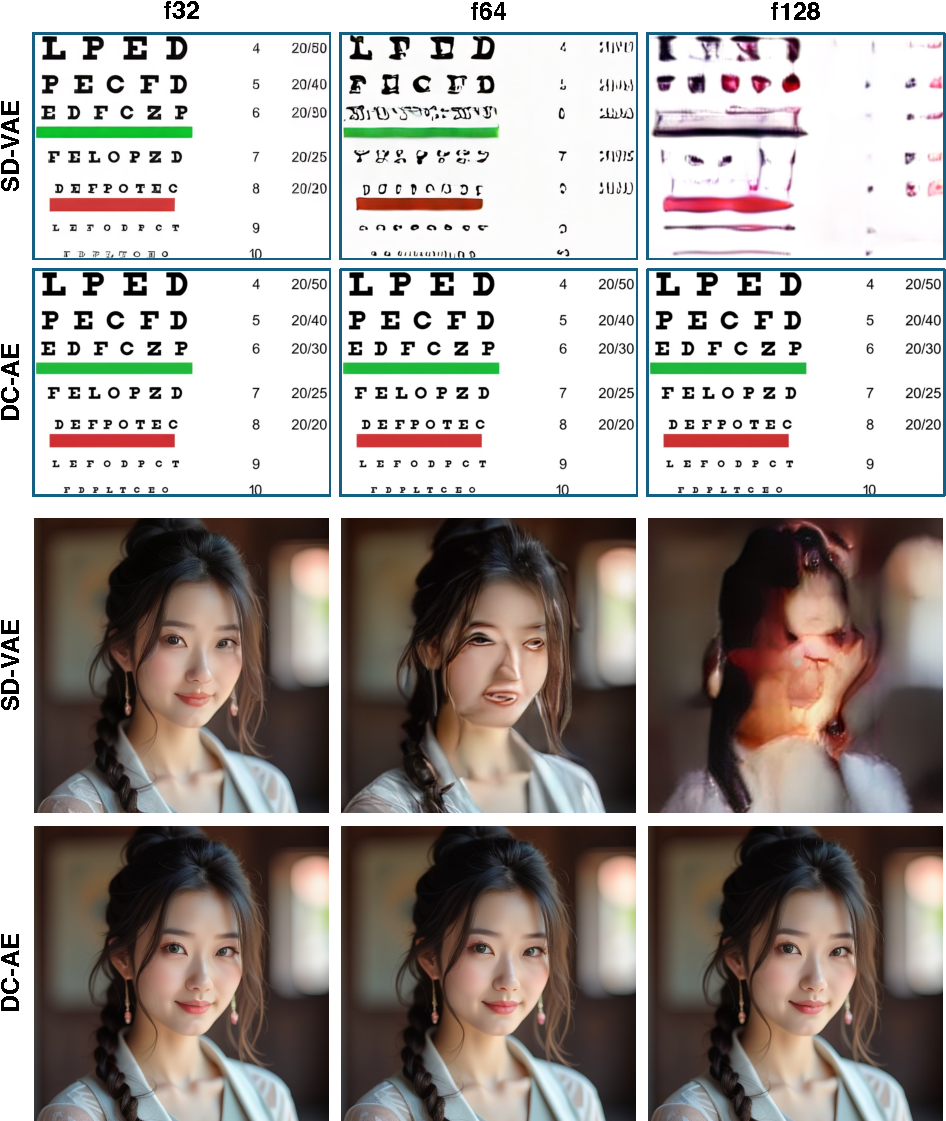
\includegraphics[width=0.95\linewidth]{figures/src/ae_visualization.pdf}
    \vspace{-10pt}
    \caption{\textbf{Autoencoder Image Reconstruction Samples.}}
    \vspace{-10pt}
    \label{fig:ae_visualization}
\end{figure}


\begin{figure}[t]
    \centering
    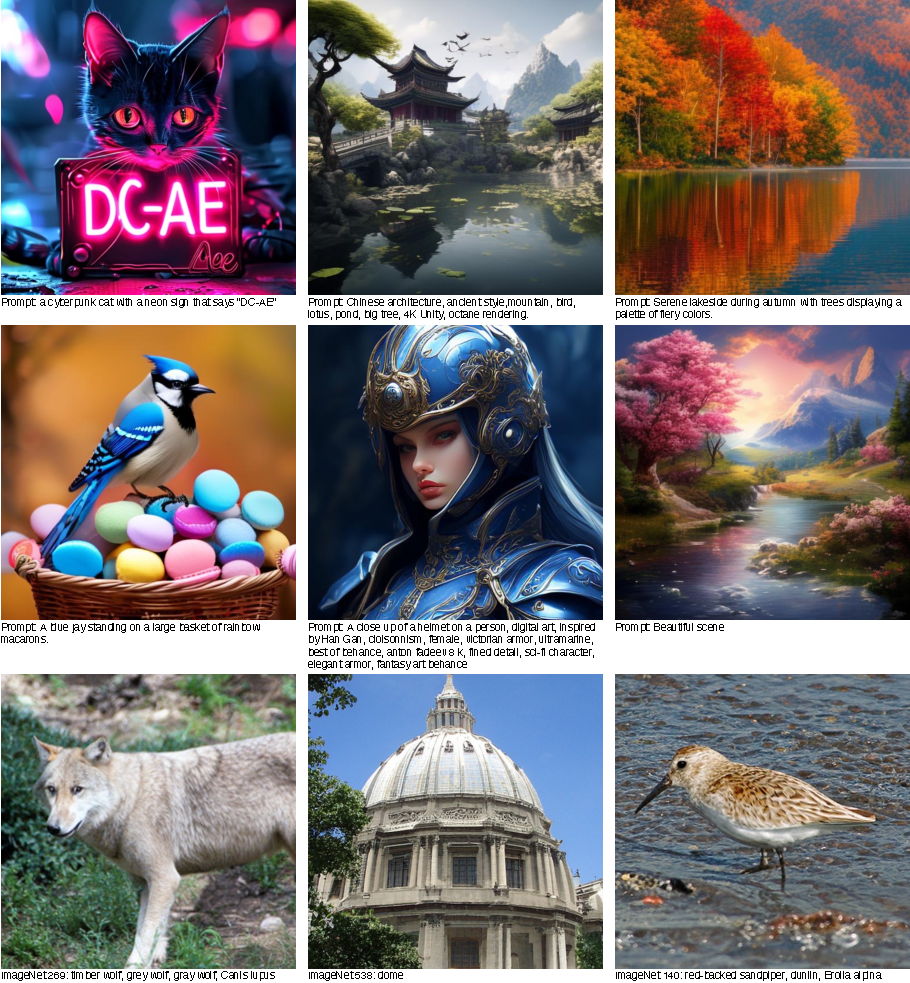
\includegraphics[width=1\linewidth]{figures/src/diffusion_visualization.pdf}
    \vspace{-15pt}
    \caption{\textbf{Images Generated by Diffusion Model using Our \modelshort.}}
    \vspace{-10pt}
    \label{fig:diffusion_visualization}
\end{figure}


\paragraph{Efficiency Profiling.} We profile the training and inference throughput on the H100 GPU with PyTorch and TensorRT respectively. The latency is measured on the 3090 GPU with batch size 2. The training memory is profiled using PyTorch, assuming a batch size of 256. We use fp16 for all cases. For simplicity, we assume the number of sampling steps is 1.

\subsection{Image Compression and Reconstruction}
Table~\ref{tab:ae_main} summarizes the results of \modelshort and SD-VAE \citep{rombach2022high} under various settings (f represents the spatial compression ratio and c denotes the number of latent channels). \modelshort provides significant reconstruction accuracy improvements than SD-VAE for all cases. For example, on ImageNet $512 \times 512$, \modelshort improves the rFID from 16.84 to 0.22 for the f64c128 autoencoder and 100.74 to 0.23 for the f128c512 autoencoder. 

In addition to the quantitative results, Figure~\ref{fig:ae_visualization} shows image reconstruction samples produced by SD-VAE and \modelshort. Reconstructed images by \modelshort demonstrate a better visual quality than SD-VAE's reconstructed images. In particular, for the f64 and f128 autoencoders,  \modelshort still maintains a good visual quality for small text and the human face. 

\subsection{Latent Diffusion Models}
We compare \modelshort with the widely used SD-VAE-f8 autoencoder \citep{rombach2022high} on various diffusion transformer models. For \modelshort, we always use a patch size of 1 (denoted as p1). For SD-VAE-f8, we follow the common setting and use a patch size of 2 or 4 (denoted as p2, p4). The results are summarized in Table~\ref{tab:diffusion_imagenet_main}, Table~\ref{tab:diffusion_hr_main}, and Table~\ref{tab:diffusion_t2i_main}. 

\vspace{-5pt}
\paragraph{ImageNet 512$\times$512.} As shown in Table~\ref{tab:diffusion_imagenet_main}, \modelshort-f32p1 consistently delivers better FID than SD-VAE-f8p2 on all diffusion transformer models. In addition, it has 4$\times$ fewer tokens than SD-VAE-f8p2, leading to 4.5$\times$ higher H100 training throughput and 4.8$\times$ higher H100 inference 
\begin{wrapfigure}{r}{0.35\textwidth}
  \vspace{-10pt}
  \begin{center}
    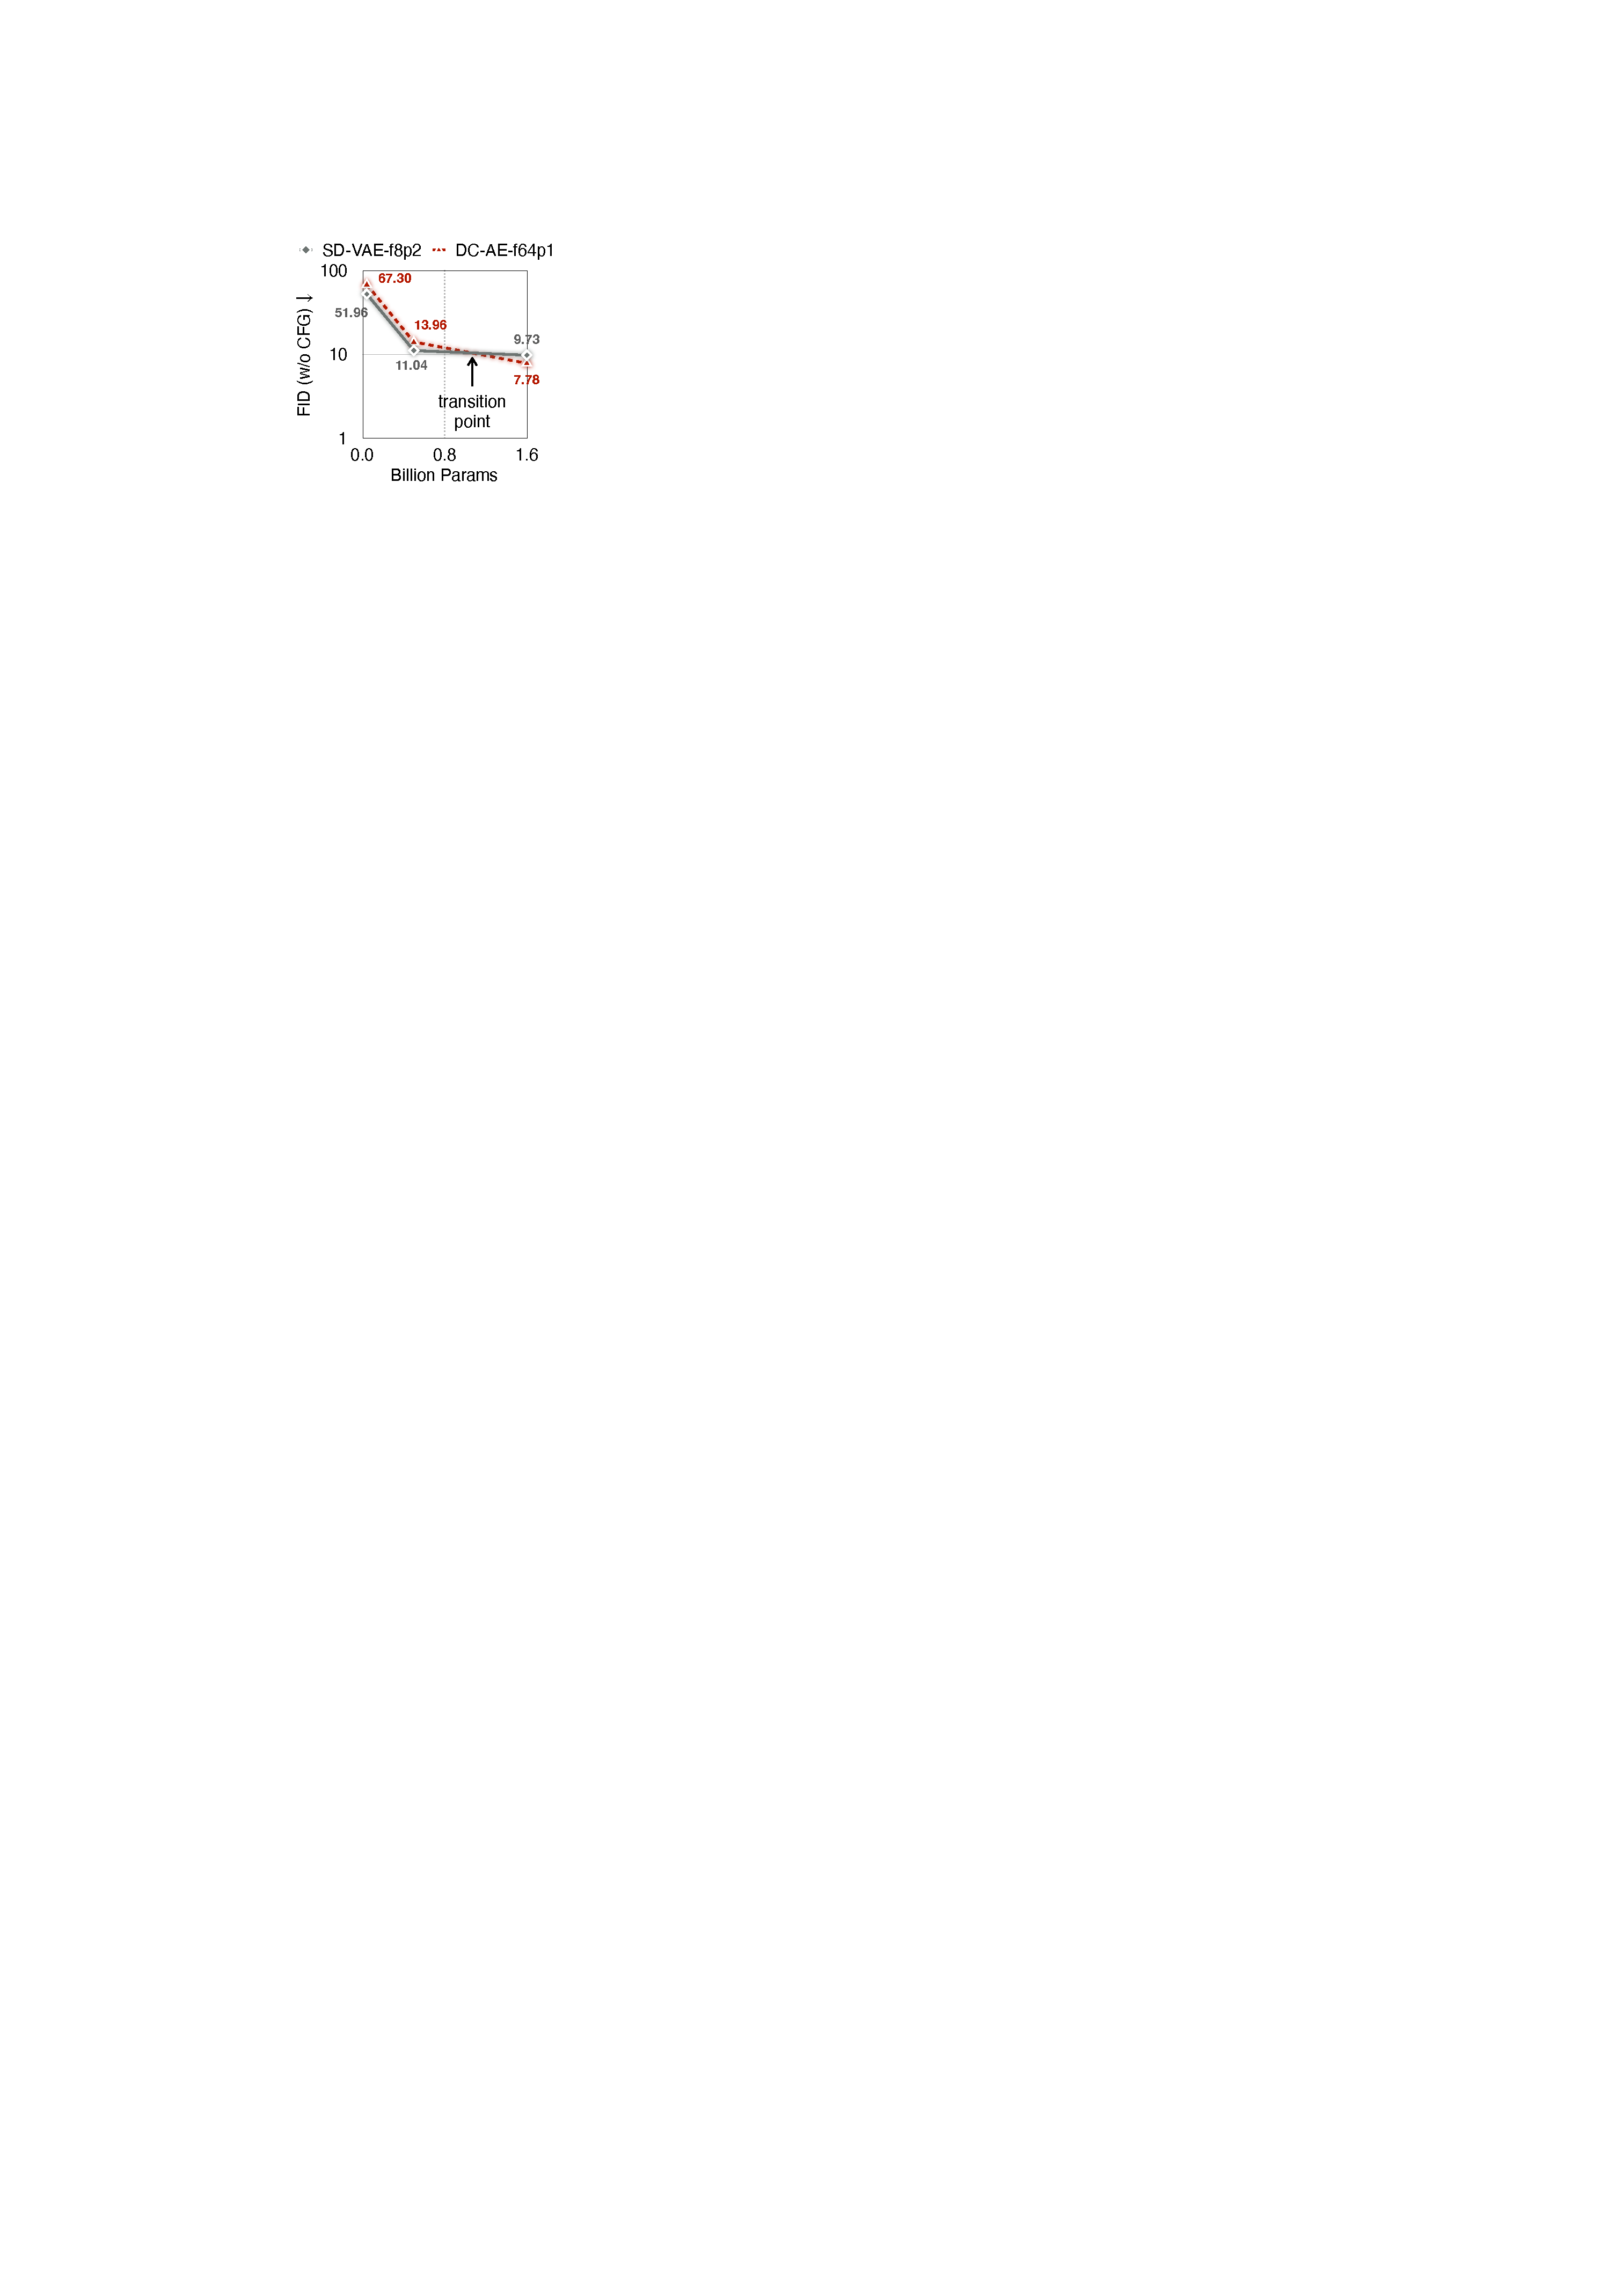
\includegraphics[width=0.35\textwidth]{figures/src/diffusion_scaling_up.pdf}
  \end{center}
  \vspace{-10pt}
  \caption{\textbf{Model Scaling Results on ImageNet 512$\times$512 with UViT.} \modelshort-f64 benefits more from scaling up than SD-VAE-f8.}
  \vspace{-20pt}
  \label{fig:diffusion_scaling_up}
\end{wrapfigure}

\!\!\!\! throughput for DiT-XL. We also observe that larger diffusion transformer models seem to benefit more from our \modelshort. For example, \modelshort-f64p1 has a worse FID than SD-VAE-f8p2 on UViT-S but a better FID on UViT-H. We conjecture it is because \modelshort-f64 has a larger latent channel number than SD-VAE-f8, thus needing more model capacity \citep{esser2024scaling}. 

\vspace{-10pt}
\paragraph{Text-to-Image Generation.} Table~\ref{tab:diffusion_t2i_main} reports our text-to-image generation results. All models are trained for 100K iterations from scratch. Similar to prior cases, we observe \modelshort-f32p1 provides a better FID and a better CLIP Score than SD-VAE-f8p2. Figure~\ref{fig:diffusion_visualization} demonstrates samples generated by the diffusion models with our \modelshort, showing the capacity to synthesize high-quality images while being significantly more efficient than prior models.
\section{Conclusion}
\label{sec:conclusion}

This paper introduces a novel approach to human image animation that integrates the SMPL 3D parametric human model with latent diffusion models, aiming to enhance pose alignment and motion guidance. 
By leveraging the unified representation of shape and pose variations offered by the SMPL model, along with depth, normal, and semantic maps, this method further improve the ability of capturing realistic human movements and shapes of previous techniques.
The inclusion of skeleton-based motion guidance and self-attention mechanisms for feature map integration further refines the animation process, enabling the creation of dynamic visual content that more accurately reflects human anatomy and movement. 
Experimental validation across various datasets confirms the effectiveness of this approach in producing high-quality human animations, showcasing its potential to advance digital content creation in fields requiring detailed and realistic human representations.


% \par\vfill\par
% Now we have reached the maximum length of an ECCV \ECCVyear{} submission (excluding references).
% References should start immediately after the main text, but can continue past p.\ 14 if needed.
% \clearpage  % TODO REVIEW/FINAL: This \clearpage needs to be removed from both review and camera-ready versions.


% ---- Bibliography ----
%
% BibTeX users should specify bibliography style 'splncs04'.
% References will then be sorted and formatted in the correct style.
%
\bibliographystyle{splncs04}
\bibliography{main}
\end{document}
